\section{Dobór parametrów regulatorów PID i DMC}
Ocena jakości regulacji na podstawie rysunków przebiegów sygnałów polega na ocenie jakościowej, 
analizowane są takie kryteria jak czas regulacji czy przeregulowanie. 
Na podstawie tych kryteriów oceny dobierane są nastawy regulatora PID.

Ocena jakości regulacji ilościowa polega na wyznaczaniu wskaźnika jakości regulacji, 
którym jest suma kwadratów uchybów, a $k_{konc}$ oznacza ilość kroków symulacji. 



$$
E=\sum_{k=1}^{k_{konc}} \quad (y_{zad}(k)-y(k))^{2}
$$

Ocena jakości regulacji jakościowa jest metodą mniej dokładną od oceny ilościowej, 
nie występują tam obliczenia a jedynie analiza rysunków przebiegów. 
Podczas analizy rysunku osoba oceniająca jakość regulacji narażona jest na mało precyzyjne wnioski, 
gdyż należy wtedy zwracać uwagę na skalę rysunku i wiele innych parametrów. 
Ocena ilościowa nie bierze pod uwagę takich czynników jak np. oscylacje, 
jedynym kryterium jest suma kwadratów uchybów. 
Jeżeli do oceny jakości regulacji wymagane są inne kryteria niż podany wskaźnik jakości 
należy rozpatrzeć metodę oceny jakościowej.

\subsection{Regulator PID}

Do doboru nastaw regulatora PID zastosowano metodę inżynierską, 
która polega na przeprowadzeniu doświadczeń i analizy uzyskanych wyników. 
Na podstawie wyciągniętych wniosków modyfikowane są nastawy regulatora. 
Parametry  dobierane są metodą prób i błędów, aż do osiągnięcia oczekiwanych wyników. 
Jako pierwszy dobierany był parametr wzmocnienia członu proporcjonalnego, 
poprzez obserwację zachowania się uchybu regulacji w stanie ustalonym oraz przeregulowanie. 
Zmniejszając stopniowo wzmocnienie zmniejszano przeregulowanie, a uchyb zwiększał się. 
Parametr  zwiększając go co likwidowało uchyb regulacji,  
zbyt duży czas zdwojenia zwiększał czas regulacji. 
Ostatnim elementem strojenia jest wyznaczenie parametru czasu wyprzedzenia , 
również metodą prób i błędów, tak by zminimalizować czas regulacji. 
Po wykonaniu tej czynności kończy się proces strojenia regulatora.


\begin{figure}[H]
    \centering
    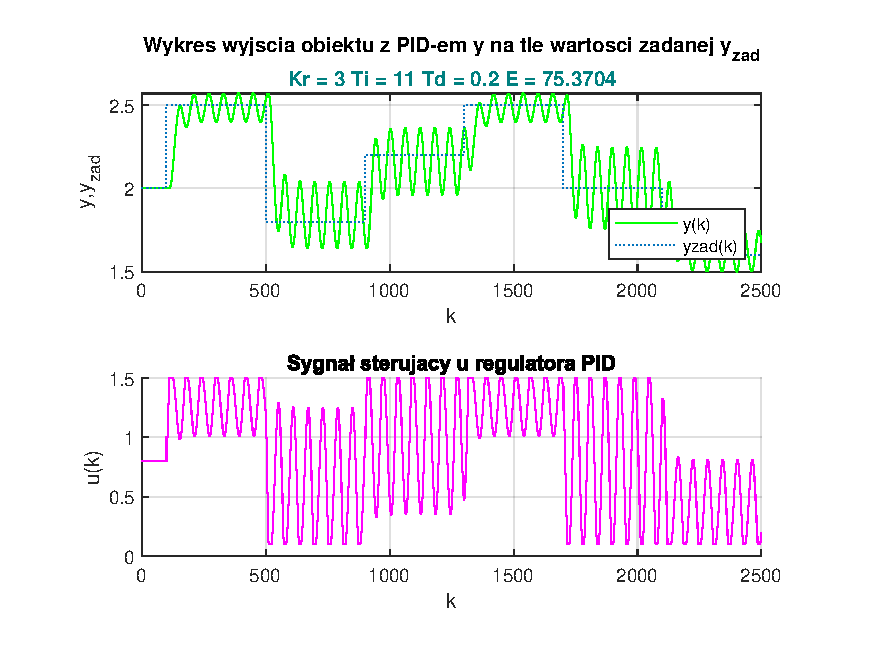
\includegraphics[scale=0.90]{../projekt/zad4_5/PID_pdf/PID_1.pdf}
    \caption{Przebiegi symulacji z danym regulatorem PID}
\end{figure}

\begin{figure}[H]
    \centering
    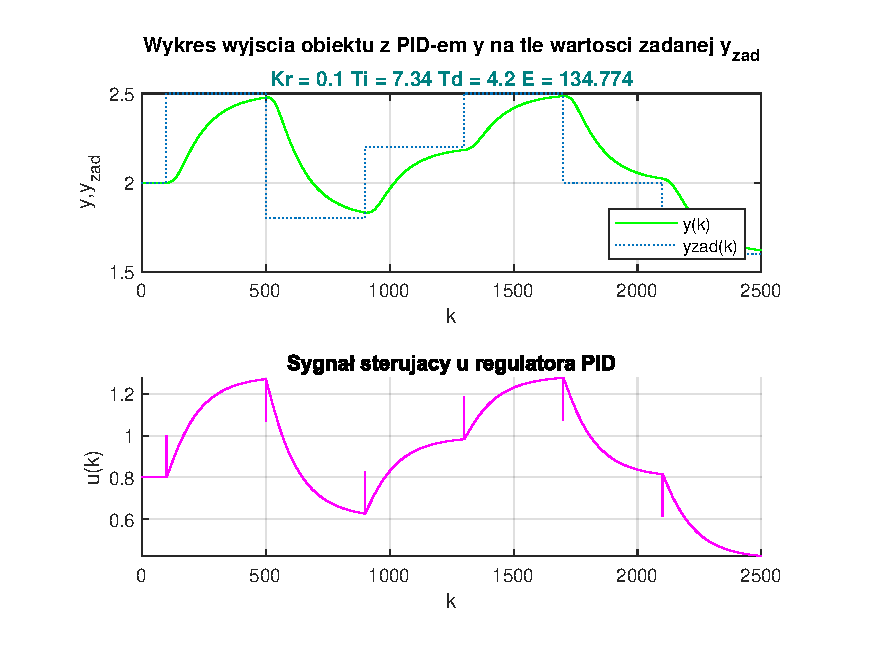
\includegraphics[scale=0.90]{../projekt/zad4_5/PID_pdf/PID_2.pdf}
    \caption{Przebiegi symulacji z danym regulatorem PID}
\end{figure}

\begin{figure}[H]
    \centering
    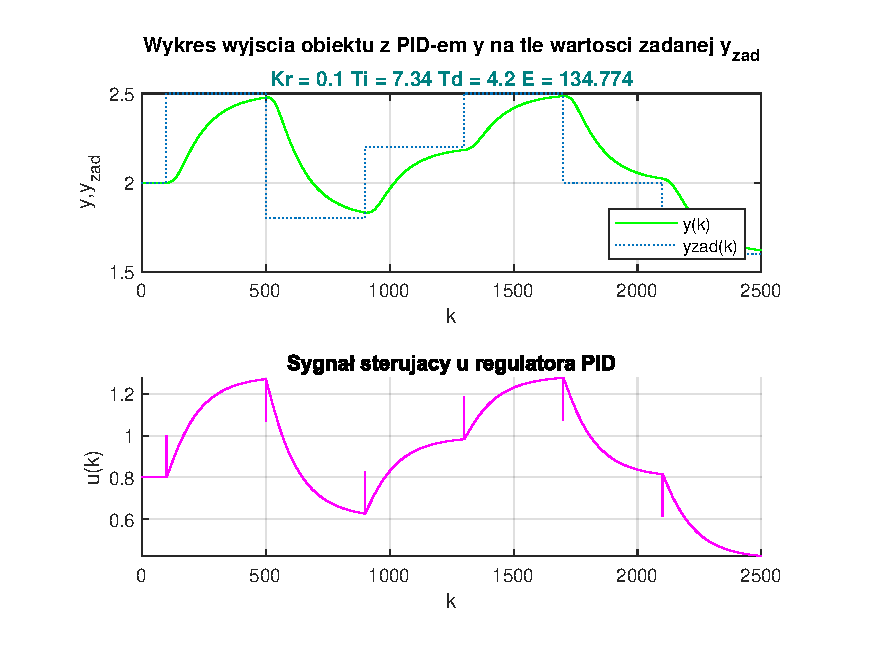
\includegraphics[scale=0.90]{../projekt/zad4_5/PID_pdf/PID_2.pdf}
    \caption{Przebiegi symulacji z danym regulatorem PID}
\end{figure}

\begin{figure}[H]
    \centering
    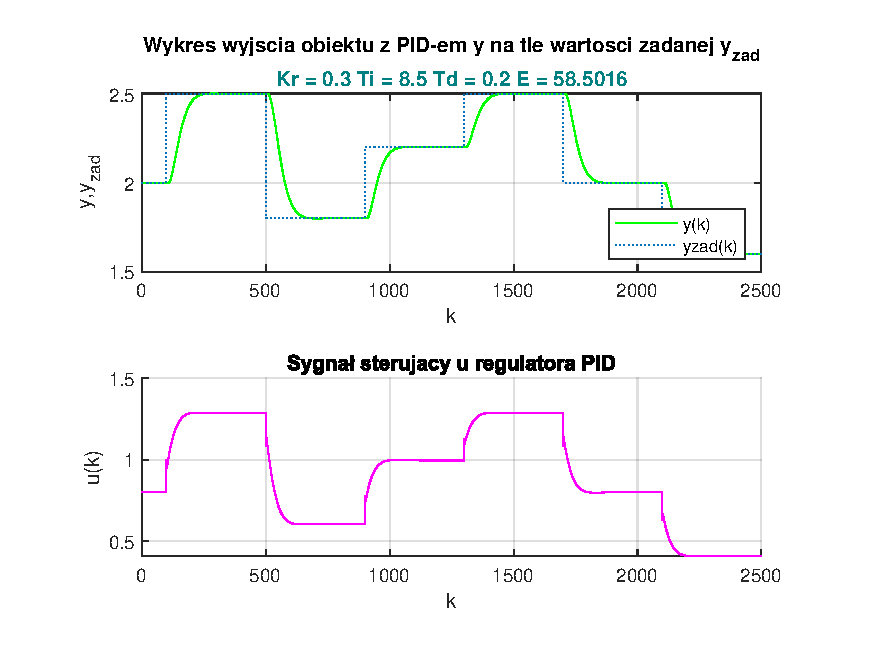
\includegraphics[scale=0.90]{../projekt/zad4_5/PID_pdf/PID_best.pdf}
    \caption{Przebiegi symulacji z najlepszym uzyskanym regulatorem PID}
\end{figure}

\subsection{Regulator DMC}

Do doboru nastaw regulatora DMC zastosowano metodę inżynierską, 
która polega na przeprowadzeniu doświadczeń i analizy uzyskanych wyników. 
Na podstawie wyciągniętych wniosków modyfikowane są nastawy regulatora. 
Parametry  dobierane są metodą prób i błędów, aż do osiągnięcia oczekiwanych wyników.

\indent Horyzont dynamiki $D$ jest to liczba współczynników odpowiedzi skokowej, 
tzn. liczbę kroków dyskretyzacji, po której można uznać odpowiedź skokową za stabilną równą $K_{stat}$. 
Wyznaczona ona została z odpowiedzi skokowej obiektu poprzez wyznaczenie z niej chwili, 
w której odpowiedź jest stabilna.

\indent Horyzont predykcji $N$ jest to wartość na podstawie, 
której prognozuje się zachowanie modelu. 
Zwiększając ten parametr uzyskaliśmy bardzo dobry czas regulacji oraz praktycznie zerowe przesterowanie.

\indent Horyzont sterowania $N_{u}$ tak jak horyzont predykcji jest parametrem dostrajania regulatora, 
zależnymi od szybkości dynamiki procesu, możliwości obliczeniowych oraz dokładności modelu, 
eksperymentalnie dobrano wartość tero parametru.

Ostatnim krokiem w dostrajaniu naszego regulatora było wyznaczenie współczynnika kary lambda, 
za pomocą którego można zapewnić kompromis pomiędzy szybkością regulacji, a postacią sygnału sterującego. 
Ponownie był on wyznaczany metodą testowania. 
Zwiększenie współczynnika kary pogorszyło wynik działania regulatora, został więc on zmniejszony.


\begin{figure}[H]
    \centering
    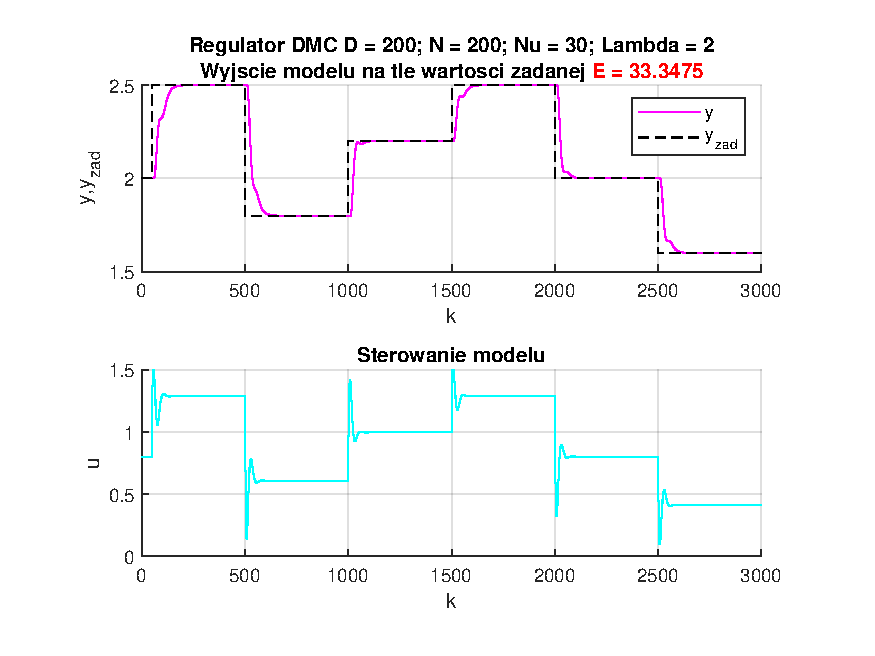
\includegraphics[scale=0.90]{../projekt/zad4_5/DMC_pdf/DMC_1.pdf}
    \caption{Przebiegi symulacji z danym regulatorem DMC}
\end{figure}

\begin{figure}[H]
    \centering
    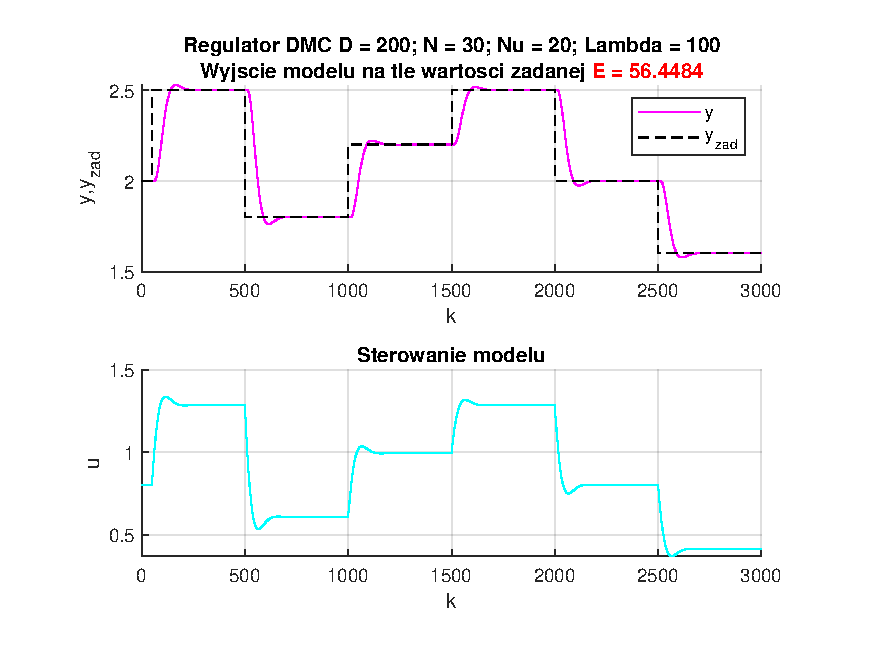
\includegraphics[scale=0.90]{../projekt/zad4_5/DMC_pdf/DMC_2.pdf}
    \caption{Przebiegi symulacji z danym regulatorem DMC}
\end{figure}

\begin{figure}[H]
    \centering
    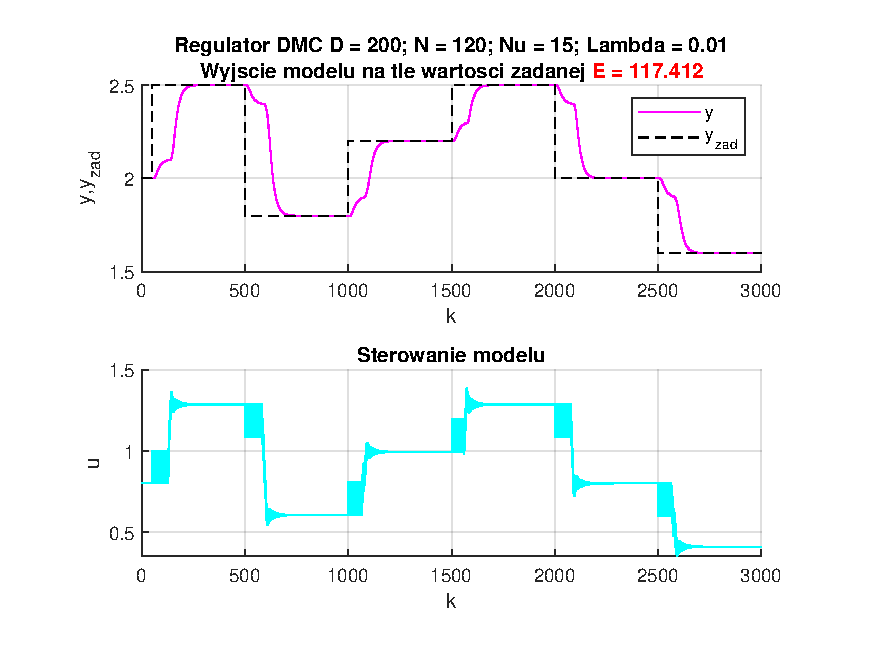
\includegraphics[scale=0.90]{../projekt/zad4_5/DMC_pdf/DMC_3.pdf}
    \caption{Przebiegi symulacji z danym regulatorem DMC}
\end{figure}

\begin{figure}[H]
    \centering
    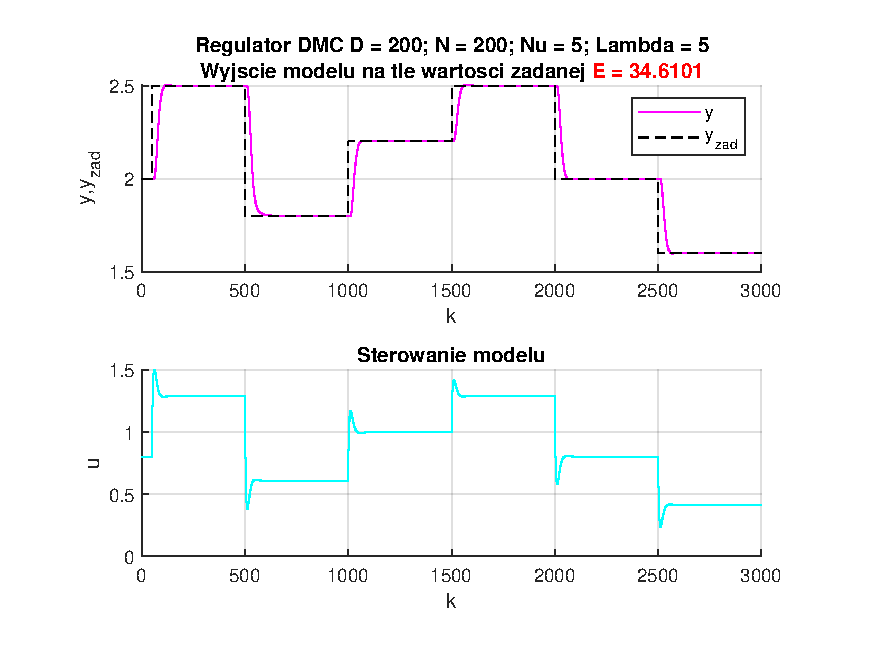
\includegraphics[scale=0.90]{../projekt/zad4_5/DMC_pdf/DMC_best.pdf}
    \caption{Przebiegi symulacji z najlepszym uzyskanym regulatorem DMC}
\end{figure}


